\documentclass[a4paper, 12pt]{article}

% --- PACKAGES ---
\usepackage{amsmath} % For math environments
\usepackage{geometry} % For page margins
\geometry{a4paper, margin=1in}
\usepackage{graphicx}
\usepackage{hyperref}
\usepackage{tikz}
\usetikzlibrary{shapes, arrows, positioning}

% --- TITLE ---
\title{Relative Position Control for Quadruped Robot \\ (Hierarchical Control Architecture)}
\author{Theerachot Mueangchamnong}
\date{February 5, 2026}

% --- DOCUMENT ---
\begin{document}

\maketitle

\section{Control System Overview}
This document describes the Hierarchical Control Architecture for Relative Position Control of a Quadruped robot along the Y-axis (forward/backward movement).

\subsection{Hierarchical Control Structure}
\textit{Description:} The control system is divided into 3 layers based on operating frequency and abstraction level. Each layer has specific responsibilities and communicates through well-defined interfaces.

\begin{center}
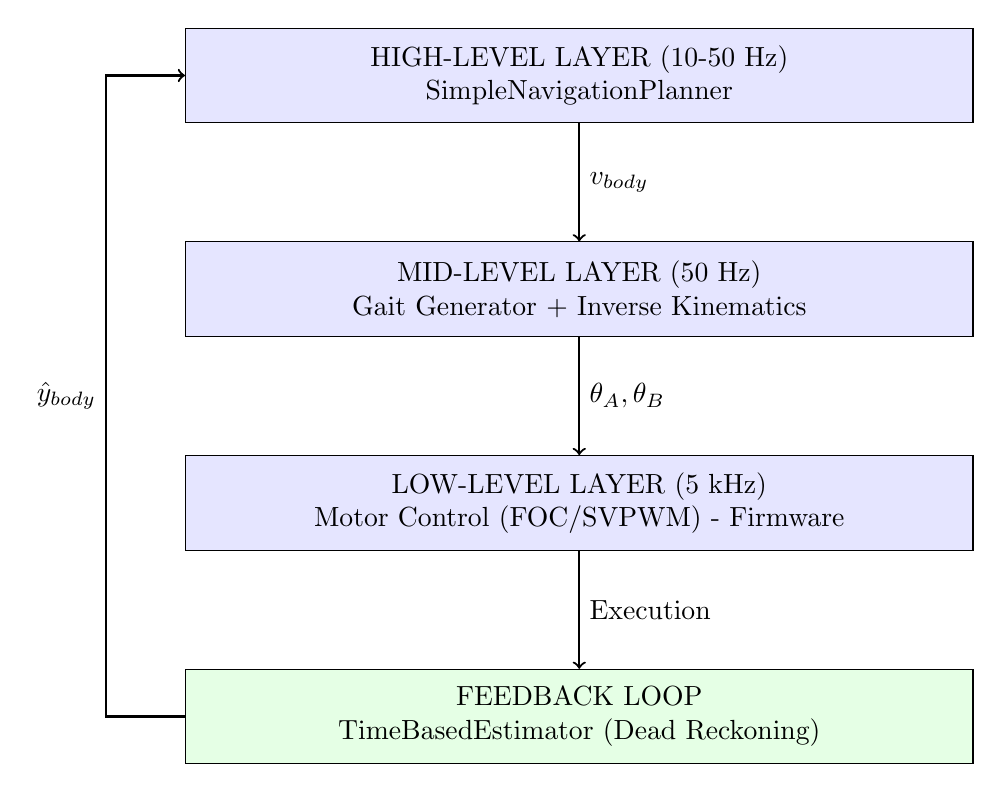
\begin{tikzpicture}[
    node distance=1.5cm,
    layer/.style={rectangle, draw, minimum width=10cm, minimum height=1.2cm, align=center, fill=blue!10},
    arrow/.style={->, thick}
]
    % Layers
    \node[layer] (high) {HIGH-LEVEL LAYER (10-50 Hz) \\ SimpleNavigationPlanner};
    \node[layer, below=of high] (mid) {MID-LEVEL LAYER (50 Hz) \\ Gait Generator + Inverse Kinematics};
    \node[layer, below=of mid] (low) {LOW-LEVEL LAYER (5 kHz) \\ Motor Control (FOC/SVPWM) - Firmware};
    \node[layer, below=of low, fill=green!10] (feedback) {FEEDBACK LOOP \\ TimeBasedEstimator (Dead Reckoning)};
    
    % Arrows
    \draw[arrow] (high) -- (mid) node[midway, right] {$v_{body}$};
    \draw[arrow] (mid) -- (low) node[midway, right] {$\theta_A, \theta_B$};
    \draw[arrow] (low) -- (feedback) node[midway, right] {Execution};
    \draw[arrow] (feedback.west) -- ++(-1,0) |- (high.west) node[near start, left] {$\hat{y}_{body}$};
\end{tikzpicture}
\end{center}

\subsection{Operating Frequencies}
\textit{Principle:} Each layer operates at a frequency appropriate to its function.

\begin{itemize}
    \item \textbf{High-Level (10-50 Hz):} Path planning, high-level decision making
    \item \textbf{Mid-Level (50 Hz):} Gait pattern generation and IK computation
    \item \textbf{Low-Level (5 kHz):} Real-time motor control (FOC/SVPWM)
    \item \textbf{Feedback:} Continuous position estimation
\end{itemize}

\section{Layer 1: High-Level Control (Navigation Planner)}
\textit{Objective:} Compute desired velocity ($v_{body}$) to move the robot to the target position.

\subsection{Simple Navigation Planner}
\textbf{Principle:} Uses a Proportional Controller (P-Controller) to compute velocity from position error.

\textbf{Inputs:}
\begin{itemize}
    \item $y_{target}$ - Target position on Y-axis (mm)
    \item $y_{current}$ - Current position from estimator (mm)
\end{itemize}

\textbf{Outputs:}
\begin{itemize}
    \item $v_{body,y}$ - Desired velocity on Y-axis (mm/s)
\end{itemize}

\subsection{Control Equations}
\textit{P-Controller:} Compute velocity from position error.

Position error:
\begin{equation}
    e_y = y_{target} - y_{current}
\end{equation}

Desired velocity (before saturation):
\begin{equation}
    v_{desired} = K_p \cdot e_y
\end{equation}

Saturated velocity:
\begin{equation}
    v_{body,y} = \text{clip}(v_{desired}, -v_{max}, +v_{max})
\end{equation}

where:
\begin{itemize}
    \item $K_p = 1.0$ - Proportional gain
    \item $v_{max} = 50$ mm/s - Maximum velocity (conservative for safety)
\end{itemize}

\subsection{Stopping Condition}
\textit{Criterion:} The robot reaches the target when

\begin{equation}
    |e_y| < \epsilon_{tolerance}
\end{equation}

where $\epsilon_{tolerance} = 10$ mm

\subsection{Tunable Parameters}
\textbf{Performance Tuning:}

\begin{itemize}
    \item \textbf{$v_{max}$:} Increase for faster movement (watch stability)
    \item \textbf{$K_p$:} Increase for faster response (watch overshoot)
    \item \textbf{$\epsilon_{tolerance}$:} Decrease for higher precision (longer time)
    \item \textbf{Timeout:} Maximum execution time limit (60 seconds)
\end{itemize}

\section{Layer 2: Mid-Level Control (Gait Generator)}
\textit{Objective:} Convert desired velocity to gait parameters and compute joint positions via Inverse Kinematics.

\subsection{Gait-to-Velocity Mapping}
\textbf{Principle:} Convert body velocity ($v_{body,y}$) to gait parameters (step length and direction).

\textbf{Gait Cycle Time:}
\begin{equation}
    T_{gait} = \frac{N_{steps}}{f_{update}}
\end{equation}

where:
\begin{itemize}
    \item $N_{steps} = $ Number of steps in one gait cycle
    \item $f_{update} = 50$ Hz - Update frequency
\end{itemize}

\textbf{Step Length:}
\begin{equation}
    L_{step} = |v_{body,y}| \cdot T_{gait}
\end{equation}

\textbf{Step Length Saturation:}
\begin{equation}
    L_{step} = \min(L_{step}, L_{step,max})
\end{equation}

where $L_{step,max}$ is the maximum step length achievable by the 5-bar mechanism.

\subsection{Walking Direction}
\textit{Description:} Walking direction is determined by the velocity sign.

\begin{equation}
    \text{reverse} = 
    \begin{cases}
        \text{True} & \text{if } v_{body,y} < 0 \text{ (backward)} \\
        \text{False} & \text{if } v_{body,y} \geq 0 \text{ (forward)}
    \end{cases}
\end{equation}

\subsection{Elliptical Trajectory Generation}
\textbf{Principle:} Generate elliptical foot trajectory for each leg.

\textbf{Parameters:}
\begin{itemize}
    \item $h_{lift}$ - Foot lift height (mm)
    \item $L_{step}$ - Step length (mm)
    \item $r_{stance}$ - Stance phase ratio (0-1)
    \item $(x_{home}, y_{home})$ - Home stance position
\end{itemize}

\textbf{Foot Trajectory:} Divided into 2 phases

\textit{1. Stance Phase} (foot on ground):
\begin{align}
    x(t) &= x_{home} + L_{step} \left(\frac{1}{2} - \frac{t}{t_{stance}}\right) \\
    y(t) &= y_{home}
\end{align}

\textit{2. Swing Phase} (foot in air):
\begin{align}
    x(t) &= x_{home} + L_{step} \left(\frac{t - t_{stance}}{t_{swing}} - \frac{1}{2}\right) \\
    y(t) &= y_{home} + h_{lift} \sin\left(\pi \frac{t - t_{stance}}{t_{swing}}\right)
\end{align}

\subsection{Trot Gait Phase Offsets}
\textbf{Principle:} In trot gait, diagonal legs move together with the following phase offsets:

\begin{itemize}
    \item \textbf{FR (Front Right):} $\phi = 0.0$ rad (0°)
    \item \textbf{RL (Rear Left):} $\phi = 0.0$ rad (0°) - moves with FR
    \item \textbf{FL (Front Left):} $\phi = \pi$ rad (180°)
    \item \textbf{RR (Rear Right):} $\phi = \pi$ rad (180°) - moves with FL
\end{itemize}

\textbf{Step Index Calculation:}
\begin{equation}
    i_{leg} = \left\lfloor \frac{\phi_{leg}}{2\pi} \cdot N_{steps} \right\rfloor \mod N_{steps}
\end{equation}

\subsection{Inverse Kinematics}
\textit{Objective:} Convert foot position $(x_f, y_f)$ to motor angles $(\theta_A, \theta_B)$.

\textbf{Input:} Foot position in leg frame
\begin{equation}
    \mathbf{P}_f = \begin{bmatrix} x_f \\ y_f \end{bmatrix}
\end{equation}

\textbf{Output:} Motor angles
\begin{equation}
    \boldsymbol{\theta} = \begin{bmatrix} \theta_A \\ \theta_B \end{bmatrix}
\end{equation}

\textit{Note:} Detailed IK calculation is described in Phase1.2\_Inverse\_Kinematics\_Analytical.tex

\section{Layer 3: Low-Level Control (Motor Control)}
\textit{Objective:} Control motors to desired angles using Field-Oriented Control (FOC).

\subsection{Angle Command Transmission}
\textbf{Unit Conversion:} From radians to degrees
\begin{equation}
    \theta_{deg} = \theta_{rad} \cdot \frac{180}{\pi}
\end{equation}

\textbf{Communication Protocol:} Binary Protocol
\begin{itemize}
    \item \textbf{Baud Rate:} 115200
    \item \textbf{Timeout:} 50 ms (Fast Mode)
    \item \textbf{Command:} \texttt{set\_position\_direct(angle\_deg)}
\end{itemize}

\subsection{Control Modes}
\textbf{Control Mode:} Configured in firmware

\begin{itemize}
    \item \textbf{Position Control:} Position control with PID
    \item \textbf{Velocity Control:} Velocity control (not used in this mode)
    \item \textbf{Torque Control:} Torque control (not used in this mode)
\end{itemize}

\textit{Note:} Motor control system details are described in Phase4.1\_Controller\_Design.tex

\section{Feedback Loop (State Estimation)}
\textit{Objective:} Estimate robot position using Dead Reckoning.

\subsection{Time-Based Estimator}
\textbf{Principle:} Estimate position by velocity integration.

\textbf{State Variables:}
\begin{itemize}
    \item $\hat{y}$ - Estimated position (mm)
    \item $v_{current}$ - Current velocity (mm/s)
    \item $t_{last}$ - Last update time (s)
\end{itemize}

\subsection{Update Equations}
\textit{Velocity Integration:} Compute position change from velocity and time.

\begin{equation}
    \Delta t = t_{current} - t_{last}
\end{equation}

\begin{equation}
    \Delta y = v_{current} \cdot \Delta t
\end{equation}

\begin{equation}
    \hat{y}_{new} = \hat{y}_{old} + \Delta y
\end{equation}

\subsection{Dead Reckoning Limitations}
\textbf{Problem:} Drift Error Accumulation

\begin{itemize}
    \item No actual position measurement (open-loop estimation)
    \item Error accumulates over time
    \item Does not detect foot slip
\end{itemize}

\textbf{Future Improvements:}
\begin{itemize}
    \item Add IMU (Inertial Measurement Unit) for acceleration measurement
    \item Add Visual Odometry or SLAM
    \item Use Kalman Filter for multi-sensor fusion
\end{itemize}

\section{Main Control Loop}
\textit{Objective:} Integrate all layers in the main control loop.

\subsection{Control Algorithm}
\textbf{Pseudocode:}

\begin{verbatim}
function move_relative_y(target_distance):
    // Initialization
    planner.set_target(target_distance)
    estimator.start()
    
    // Main loop
    while not planner.is_target_reached():
        // 1. High-Level: Compute velocity
        v_body = planner.compute_velocity()
        
        // 2. Mid-Level: Generate trajectories
        for each leg:
            trajectory[leg] = get_trajectory(v_body, leg_id)
            foot_pos = trajectory[leg][step_index]
            
            // 3. Mid-Level: Inverse Kinematics
            (theta_A, theta_B) = compute_IK(foot_pos)
            
            // 4. Low-Level: Send to motors
            send_to_motors(theta_A, theta_B)
            
            // Advance step index
            step_index = (step_index + 1) mod N_steps
        
        // 5. Feedback: Update position estimator
        estimator.update(v_body, current_time)
        y_estimated = estimator.get_position()
        
        // 6. Close loop
        planner.update_position(y_estimated)
        
        // Wait for next cycle
        sleep(1 / f_update)
    
    return SUCCESS
\end{verbatim}

\subsection{Operating Frequency}
\textbf{Main Loop Frequency:} $f_{update} = 50$ Hz

\textbf{Loop Timing:}
\begin{equation}
    T_{loop} = \frac{1}{f_{update}} = \frac{1}{50} = 0.02 \text{ s} = 20 \text{ ms}
\end{equation}

\textbf{Time Management:} Use sleep to maintain constant loop frequency.

\begin{equation}
    t_{sleep} = T_{loop} - t_{computation}
\end{equation}

\section{Testing and Results}
\textit{Objective:} Verify control system correctness.

\subsection{Test Cases}
\textbf{Test Suite:}

\begin{enumerate}
    \item \textbf{Short Forward:} Move forward +100 mm
    \item \textbf{Short Backward:} Move backward -100 mm
    \item \textbf{Long Forward:} Move forward +500 mm
\end{enumerate}

\subsection{Evaluation Metrics}
\textbf{Performance Indicators:}

\begin{itemize}
    \item \textbf{Position Error:} $e_{final} = |y_{target} - y_{final}|$
    \item \textbf{Time to Target:} $t_{total}$
    \item \textbf{Average Velocity:} $\bar{v} = \frac{y_{final}}{t_{total}}$
    \item \textbf{Success Rate:} Percentage reaching target within tolerance
\end{itemize}

\subsection{Operating Modes}
\textbf{Hardware Mode:} Using real motors
\begin{itemize}
    \item Requires 8 motors connected (4 legs × 2 motors)
    \item Uses Binary Protocol to communicate with firmware
\end{itemize}

\textbf{Simulation Mode:} Software simulation
\begin{itemize}
    \item Used when hardware is unavailable
    \item Tests algorithms and logic
    \item Displays output via console
\end{itemize}

\section{Conclusion}
\subsection{Advantages of Hierarchical Architecture}
\begin{itemize}
    \item \textbf{Modularity:} Each layer works independently, easy to develop and test separately
    \item \textbf{Scalability:} Can add new features without affecting other layers
    \item \textbf{Separation of Concerns:} Clear separation of planning, gait generation, and motor control
    \item \textbf{Real-time Performance:} Each layer operates at appropriate frequency
\end{itemize}

\subsection{Limitations and Future Development}
\textbf{Current Limitations:}
\begin{itemize}
    \item Dead Reckoning has drift error
    \item Only controls Y-axis (forward/backward)
    \item No obstacle detection
    \item Maximum velocity limited for safety
\end{itemize}

\textbf{Future Development:}
\begin{itemize}
    \item Add 2D control (X-Y movement)
    \item Add IMU and sensor fusion
    \item Develop more sophisticated path planning
    \item Add obstacle detection and avoidance
    \item Improve gait for higher speeds
\end{itemize}

\section{References}
\begin{itemize}
    \item Phase1.1\_Forward\_Kinematics\_5Bar.tex - Forward Kinematics
    \item Phase1.2\_Inverse\_Kinematics\_Analytical.tex - Inverse Kinematics
    \item Phase4.1\_Controller\_Design.tex - Motor Control Design
    \item Python Implementation: relative\_position\_control.py
\end{itemize}

\end{document}
